%Copyright 2014 Jean-Philippe Eisenbarth
%This program is free software: you can 
%redistribute it and/or modify it under the terms of the GNU General Public 
%License as published by the Free Software Foundation, either version 3 of the 
%License, or (at your option) any later version.
%This program is distributed in the hope that it will be useful,but WITHOUT ANY 
%WARRANTY; without even the implied warranty of MERCHANTABILITY or FITNESS FOR A 
%PARTICULAR PURPOSE. See the GNU General Public License for more details.
%You should have received a copy of the GNU General Public License along with 
%this program.  If not, see <http://www.gnu.org/licenses/>.

%Based on the code of Yiannis Lazarides
%http://tex.stackexchange.com/questions/42602/software-requirements-specification-with-latex
%http://tex.stackexchange.com/users/963/yiannis-lazarides
%Also based on the template of Karl E. Wiegers
%http://www.se.rit.edu/~emad/teaching/slides/srs_template_sep14.pdf
%http://karlwiegers.com
\documentclass{scrreprt}
\usepackage{listings}
\usepackage{underscore}
\usepackage[bookmarks=true]{hyperref}
\usepackage[utf8]{inputenc}
\usepackage[english]{babel}
\usepackage{tocbibind}
\usepackage{graphicx}
\usepackage{svg}
\usepackage{tabularx}
\hypersetup{
    bookmarks=false,    % show bookmarks bar?
    pdftitle={Software Requirement Specification},    % title
    pdfauthor={Jean-Philippe Eisenbarth},                     % author
    pdfsubject={TeX and LaTeX},                        % subject of the document
    pdfkeywords={TeX, LaTeX, graphics, images}, % list of keywords
    colorlinks=true,       % false: boxed links; true: colored links
    linkcolor=blue,       % color of internal links
    citecolor=black,       % color of links to bibliography
    filecolor=black,        % color of file links
    urlcolor=purple,        % color of external links
    linktoc=page            % only page is linked
}%
\def\myversion{1.0 }
\date{}
%\title
\usepackage{hyperref}

\DeclareOldFontCommand{\bf}{\normalfont\bfseries}{\mathbf}

\begin{document}

\newcounter{usecaseid}[section] % Make the counter local to subsections
\newcommand{\usecaseid}{\stepcounter{usecaseid}UC\thesection.\theusecaseid}


\newcounter{freqid}[section] % Make the counter local to subsections
\newcommand{\freqid}{\stepcounter{freqid}FREQ\thesection.\thefreqid. }



\pagenumbering{gobble}
\begin{flushright}
    \rule{16cm}{5pt}\vskip1cm
    \begin{bfseries}
        \Huge{SOFTWARE REQUIREMENTS\\ SPECIFICATION}\\
        \vspace{1cm}
        for\\
        \vspace{1cm}
        $<$HUFS Calculator$>$\\
        \vspace{1cm}
        \LARGE{Version \myversion}\\
        \vspace*{\fill}
        \textit{Prepared by:}\\
            John Doe\\
            Gil Dong Hong\\
        \vspace{1cm}
        XYZ SOFTWARES\\
        \vspace{1cm}
        \today\\
    \end{bfseries}
\end{flushright}

\tableofcontents


\chapter{Introduction}
\pagenumbering{arabic}

\section{Purpose}
This Software Requirements Specification (SRS) document defines the functional and non-functional requirements for an online calculator application. The calculator will be used by students and teachers within Hankuk University of Foreign Studies (HUFS) to perform complex mathematical calculations. This SRS covers all aspects of the calculator application, including user interface, functionality, performance, and security.


\section{Document Conventions}
\subsection*{Font Conventions}
\begin{itemize} 
    \item Bold: Used to highlight keywords and important terms.
    \item Italics: Used to emphasize specific points or to introduce new concepts.
\end{itemize}
\subsection*{Requirement Prioritization}
Requirements are prioritized using a three-tier system: High, Medium, and Low.
Lower-level requirements are assumed to inherit the priority of their parent requirements unless explicitly specified otherwise.

\section{Intended Audience and Reading Suggestions}
This SRS is intended for the following audiences:
\begin{itemize}
    \item Developers: To understand the functional and non-functional requirements of the calculator application.
    \item Project Managers: To track project progress and manage resources.
    \item Testers: To develop test cases and conduct testing activities.
    \item System Administrators: To deploy and maintain the calculator application.
\end{itemize}
To understand the overall scope and objectives of the project, it is recommended to read the "Overall Description" (Section~\ref{sec:overall}) section first. Then, readers can focus on the specific sections that are relevant to their roles and responsibilities.

\section{Project Scope}

The online calculator application will provide students and teachers with a powerful tool to perform complex mathematical calculations. The system will:
\begin{itemize}
    \item Authenticate users using the school's existing authorization system.
    \item Provide a user-friendly interface for basic and advanced mathematical functions.
    \item Allow users to save and retrieve their calculations.
    \item Ensure the security and privacy of user data.
    \item Be accessible from various devices (desktop, tablet, mobile).
\end{itemize}
By providing these features, the calculator will enhance the learning experience for students and improve the efficiency of teaching and research activities.

\section{References}
\let\oldchapter\chapter
\let\chapter\section
\begingroup
\renewcommand{\chapter}[2]{}
%\renewcommand{\bibname}{ }
\begin{thebibliography}{10}
\bibitem{hufs} HUFS Authorization System (https://auth.hufs.ac.kr).

\bibitem{javaswing} Java Swing Toolkit for GUI Design

\end{thebibliography}
\endgroup

\let\chapter\oldchapter

\chapter{Overall Description}
\label{sec:overall}

\section{Product Perspective}
The online calculator is a web-based application designed to provide students and teachers with a powerful tool for performing complex mathematical calculations. It integrates with the school's existing authorization system \cite{hufs} to ensure secure access. The calculator will be deployed on the school's server infrastructure and accessed through web browsers. The following is the context diagram of the system.

\begin{center}
\includesvg{context}
%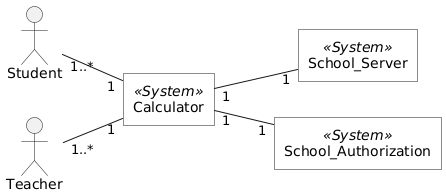
\includegraphics[scale=1.0]{context.png}
\end{center}

\section{Product Functions}
\begin{itemize}
    \item Basic Arithmetic Operations: Addition, subtraction, multiplication, and division.
    \item Advanced Mathematical Functions: Trigonometry, logarithms, exponential functions, and calculus functions.   
    \item User Authentication: Authenticate users using the school's authorization system.
    \item User Authorization: Control access to the calculator based on user roles and permissions.
    \item Data Storage: Allow users to save and retrieve their calculations.
\end{itemize}
The following is a dataflow diagram indicating a top-level view of the overall system functions. (You may also use a usecase diagram here)

\begin{center}
\includesvg{dfd}
\end{center}

\section{User Classes and Characteristics}
\subsection*{Students}
\begin{itemize}
    \item Primary users of the calculator.
    \item Varying levels of mathematical expertise.
    \item Require a user-friendly interface.
\end{itemize}
\subsection*{Teachers}
\begin{itemize}
    \item May use the calculator for demonstrations or to create assignments.
    \item Require administrative privileges to manage user access.
\end{itemize}

\section{Operating Environment}
{\bf Hardware:} School's server infrastructure\\
{\bf Operating System:} Linux or Windows Server\\
{\bf Web Server:} Apache or Nginx\\
{\bf Database:} MySQL or PostgreSQL\\
{\bf Browser Compatibility:} Chrome, Firefox, Edge, Safari\\

\section{Design and Implementation Constraints}
\begin{itemize}
    \item The calculator must integrate seamlessly with the school's existing authorization system.
    \item TBD
\end{itemize}

\section{User Documentation}

\begin{itemize}
    \item User Manual: A comprehensive user manual will be provided to guide users on how to use the calculator.
    \item Online Help: Context-sensitive help will be available within the calculator application.
\end{itemize}

\section{Assumptions and Dependencies}
\begin{itemize}
    \item The school's authorization system will be available and functioning correctly.
    \item The school's server infrastructure will have sufficient capacity to handle the load of the calculator application.
    \item The school's network will be reliable and secure.
\end{itemize}

\chapter{System Features}
\label{sec:features}
The following table summarizes the requirements listed in Section \ref{sec:features}.

\begin{center}
\begin{tabular}{|c|c|c|}

\hline
Component & Reference Number & Requirement Name\\
\hline
Comp1 & \ref{feat:1} & Req1 \\
Comp1 & \ref{feat:2} & Req2 \\
\hline

\end{tabular}
\end{center}

\section{User Authentication}
\label{feat:1}

\subsection{Description and Priority}
The system shall authenticate users using the school's existing authorization system. (Priority: high)

(\textit{Using the school's authorization system ensures secure access only to the teachers and students in the school.})

\subsection{Stimulus/Response Sequences}
\subsubsection*{User Login}
\begin{itemize}
    \item Stimulus: User enters valid credentials (username and password).
    \item Response: System verifies credentials with the school's authorization system.
    \item Response: If credentials are valid, the system grants access to the calculator.
    \item Response: If credentials are invalid, the system displays an error message.
\end{itemize}

\subsubsection*{Session Timeout}
\begin{itemize}
    \item Stimulus: User is inactive for a specified period.
    \item Response: System automatically logs the user out.
\end{itemize}

\subsection{Functional Requirements}

\begin{itemize}
    \item \freqid The system shall prompt the user to enter their username and password upon initial access.
    \item \freqid The system shall validate the user's credentials against the school's authorization system.
    \item \freqid Upon successful authentication, the system shall grant the user access to the calculator's features and functionalities.
    \item \freqid If authentication fails, the system shall display an error message and prompt the user to re-enter their credentials.
    \item \freqid The system shall maintain user sessions and automatically log out inactive users after a specified period.
\end{itemize}

\subsection{Use Cases}

\begin{tabularx}{\textwidth}{|l|X|}
\hline
\bf Use Case ID & \usecaseid \\ 
\hline
\bf Use Case Name & Student Login \\ 
\hline	
\bf Actors & Student \\
\hline	
\bf Description & The student logs into the calculator using their school credentials.\\
\hline	
\bf Trigger & Student opens the calculator application.\\
\hline	
\bf Preconditions & Student has a valid school account.\\
\hline	
\bf Postconditions & Student is logged into the calculator.\\
\hline	
\bf Normal Flow & 
Student enters their username and password.
System verifies credentials with the school's authorization system.
If credentials are valid, the system grants access to the calculator. 
\\
\hline	
\bf Alternative Flow & If credentials are invalid, the system displays an error message and prompts the user to re-enter their credentials.
\\
\hline	
\bf Exceptions & System displays an error message and logs the error if it fails to connect to the authorization system.\\
\hline	
\end{tabularx}
(See Fig~\ref{fig:seq-diagram} for the sequence diagram.)


\section{System Feature 2 (and so on)}
\label{feat:2}




\chapter{External Interface Requirements}

\section{User Interfaces}
{\bf Primary User Interface:} A graphical user interface (GUI) displayed on a digital screen, similar to a standard calculator. 

There shall also be a text field at the top of the screen, by which the user can directly type in complex equations or operations. 

{\bf Secondary User Interface:} A login screen to authenticate the user with the school's authorization system.

\section{Hardware Interfaces}
N/A

\section{Software Interfaces}
\subsubsection*{School's Authorization System}
\begin{itemize}
    \item The calculator will integrate with the school's existing authorization system to authenticate users.
    \item The system will use standard authentication protocols (e.g., OAuth, SAML) to securely exchange user information.
\end{itemize}
\subsubsection*{Database}
\begin{itemize}
    \item The calculator may use a database to store user preferences, calculation history, and other relevant data.
    \item The database will be accessed using SQL queries.
\end{itemize}


\section{Communications Interfaces}
\subsubsection*{Network Communication}
\begin{itemize}
    \item The calculator will communicate with the server over HTTP.
    \item Data will be transmitted using JSON format.
\end{itemize}

\subsubsection{Security}
\begin{itemize}
    \item HTTPS will be used to encrypt communication between the client and server.
    \item Appropriate security measures will be implemented to protect user data.
\end{itemize}


\chapter{Other Nonfunctional Requirements}

\section{Performance Requirements}

\begin{itemize}
    \item The system shall respond to user input within 2 seconds under normal load conditions.
    \item The system shall be able to handle a growing number of users without significant performance degradation. With 1000 simultaneous users, the response time should be within 3 seconds.
\end{itemize}


\section{Security Requirements}
\begin{itemize}
    \item Sensitive data, such as user passwords, shall be encrypted at rest and in transit.
\end{itemize}

\section{Software Quality Attributes}
N/A

\section{Business Rules}
\begin{itemize}
    \item Teachers can approve or deny student access to the calculator.
    \item The system shall comply with all relevant data privacy and security regulations.
\end{itemize}


\chapter{Other Requirements}

\begin{itemize}
    \item The system shall comply with all applicable laws and regulations, including data privacy laws and copyright laws.
\end{itemize}


\chapter*{Appendices}
\addcontentsline{toc}{chapter}{Appendices}
%\appendix
\renewcommand{\thesection}{\Alph{section}}

\section{Glossary}
\subsection*{Acronyms and Abbreviations}
\begin{tabularx}{\textwidth}{|l|X|}
\hline
SRS & Software Requirements Specification\\
UI & User Interface\\
HTTP & Hypertext Transfer Protocol\\
HTTPS & Hypertext Transfer Protocol Secure\\
SQL & Structured Query Language\\
JSON & JavaScript Object Notation\\
\hline
\end{tabularx}

\subsection*{Terms}
\begin{tabularx}{\textwidth}{|l|X|}
\hline
Authentication & The process of verifying a user's identity.\\
Authorization & The process of granting access to specific resources or functionalities.\\
Session & A temporary interaction between a user and a system.\\
\hline
\end{tabularx}





\section{Analysis Models}

\begin{figure}[h]
    \centering
    %\includegraphics[width=0.5\linewidth]{}
    \caption{Sequence diagram for Student Login usecase.}
    \label{fig:seq-diagram}
\end{figure}




\section{To Be Determined List}
N/A

\end{document}
